\documentclass[12pt]{article}

% --- Packages ---
\usepackage[utf8]{inputenc}
\usepackage[margin=1in]{geometry}
\usepackage{amsmath, amssymb}
\usepackage{booktabs}
\usepackage{enumitem}
\usepackage{fancyhdr}
\usepackage{float}
\usepackage{graphicx}
\usepackage{hyperref}
\usepackage{listings}
\usepackage{xcolor}

% --- References ---
% https://www.overleaf.com/learn/latex/Bibliography_management_with_biblatex
\usepackage{biblatex}
\addbibresource{references.bib}

% --- Formatting Setup ---
\hypersetup{
    colorlinks=true,
    linkcolor=blue,
    filecolor=magenta,      
    urlcolor=blue,
}

\title{CSE 554: Assignment 2}
\author{Jack Lowry, Nam Pho, Brett Saiki}
\date{February 11, 2026}

\begin{document}

\pagestyle{fancy}

\fancyhead{} % clear all header fields
\fancyhead[LO]{CSE 554: Group 14}
\fancyhead[CO]{HW2 (Winter 2026)}
\fancyhead[RO]{February 11, 2026}

\fancyfoot{} % clear all footer fields
\fancyfoot[CO]{\thepage}

\maketitle

% --- Section 1: SiLU ---
\section{Conceptual Questions}

\begin{enumerate}[label=\textbf{Q\arabic*.}]
    \item 
    \begin{enumerate}
        \item What is a KV cache in the transformer architecture? \\

        Key-Value (KV) cache is a memory optimization technique for the attention mechanism in transformers \cite{kv}. The KV cache speeds up the attention calculation by avoiding unnecessary recalculations during the autoregressive token generation process. Since the $K$ and $V$ values would be the same each pass, the computation results are cached instead of recalculated and turns a compute bound problem into a memory bound problem. \\

        \item Why is there no Q cache? \\

        When processing tokens later in the sequence, old $K$ and $V$ values depend only on the value of prior tokens, and thus can be cached. However, during attention, $Q$ is always calculated using the newest token only, and thus none of the old $Q$ values will be used during attention calculation. \\

        \item If we only perform prefill to get the first response token, which part of the computation (e.g., which layer, for which token, which operation) is not necessary? \\

        %We do not need to perform any of the decode layers since these computations only apply to response tokens beyond those generated by the prefill. \\
        To generate the first token, only the last token in the prompt is required. Specifically, the final hidden state for the last prompt token is passed into one last RMS norm and multiplied by the LM head weights to produce logits associated with the prediction of the first token. \\

        \item What is the performance implication if we apply RoPE before inserting a token into the KV cache, compared to applying RoPE after loading the KV cache and before performing attention? \\

        If we apply RoPE after loading from the KV cache, then we have to continually recompute the rotation of cached keys. The number of cached keys grows linearly with the number of tokens, so we would incur a linear overhead as it is $\mathcal{O}\left(N\right)$. Applying RoPE before caching ensures we do not need to recompute the rotation as it is $\mathcal{O}\left(1\right)$. \\

        \item If request A has input sequence [Text][Question] and request B has input sequence [Question][Text] (Questions are the same, Texts are the same, assume tokens are all unique), will they have a segment of KV cache with the same content (may be in different position) if RoPE is applied to tokens before inserting into the KV cache? If any, which part will be the same? Explain your answer in detail. \\

        No, applying RoPE makes the representation of a token dependent on its position and context relative to other tokens. Even if the [Question] and [Text] are identical in both circumstances, their relative positions change and that would result in different rotated values in KV caches. Specifically, only the keys (K) in the KV cache change since RoPE is only applied to Q and K in Llama and only K and V are in the KV cache. \\ 
        
        At a high level, the V vector should also differ between requests. The vectors in V that represent tokens are both position invariant and don't have the rotation applied and will be identical for each equivalent token. However, the way the V cache is constructed is appending the presented tokens in order. Therefore the segment of vectors in V cache representing the tokens associated with [Text] should appear first followed by by [Question] in request A but identical and swapped in request B. The underlying vectors within the V cache themselves are identical in both requests since they are token dependent and not position dependent. \\
        
        \item What if the RoPE is applied after the KV cache during the attention computation? If any, which part will be the same? Explain your answer in detail. \\

        If RoPE were applied after, then the cached keys will be the same, but in a different order. The K cache would now resemble the V cache as described in the previous question. The segments associated with [Text] and [Question] would be the same in K and V caches but swapped depending on the order these segments were received in the request.

    \end{enumerate}

    \item 
    \begin{enumerate}
        \item What is the number of floating-point computations in MLP with and without KV cache for a request with input length $p$ and output length $d$ (use $\mathcal{O}()$ notation)?\\
        
        \textbf{\underline{No KV Cache}}: Each token must be processed separately so the total FLOPs would be represented by the sum of the compute required for each individual token $T_i\ \forall i \in d$.
        \begin{align*}
            \text{FLOPs} &= T_1 + T_2 + T_3 + \cdots + T_d \\
            &= \left(p+0\right) + \left(p+1\right) + \left(p+2\right) + \cdots + \left(p+d-1\right) \\
            &= \sum_{i=0}^{d-1} p+i \\
            &= \left(\sum_{i=1}^{d} p\right) + \left( \sum_{i=1}^{d-1} i\right) \\
            &= dp + \frac{\left(d-1\right)\left(\left(d-1\right)+1\right)}{2} \\
            &= dp + \frac{d^2-d}{2}
        \end{align*}
        The complexity is $\boxed{\mathcal{O}\left(dp + d^2\right)}$ \underline{without} KV cache.\\ 

        \textbf{\underline{KV Cache}}: The total compute is the sum of two distinct phases, prefill and decode.
        \begin{align*}
            \text{FLOPs} &= \langle\text{Prefill}\rangle + \langle\text{Decode}\rangle \\
            &= p + d
        \end{align*}
        The complexity is $\boxed{\mathcal{O}\left(p+d\right)}$ \underline{with} KV cache.\\
        
        \item What is the number of floating-point computations in Attention with and without KV cache for a request input length $p$ and output length $d$ (use $\mathcal{O}\left(\right)$ notation)?
        \begin{align*}
            \text{Attention}\left(Q,K,V\right) &= \text{softmax}\left(\frac{QK^T}{\sqrt{d_k}}\right)V
        \end{align*}
        The $QK^T$ multiplication is dimension $\left(n\times h\right) \times \left(h \times n\right) \rightarrow \left(n\times n\right)$ and requires $\left(2h-1\right)n^2$ FLOPs. Dividing this attention score by a constant requires $n^2$ FLOPs. The softmax should be $\left(3n-1\right)n$ FLOPs. The final multiplication with $V$ is $\left(n\times n\right) \times \left(n\times h \right) \rightarrow \left(n\times h\right)$ and would require $\left(2n-1\right)nh$ FLOPs. In this worked example, $n$ represents the input dimension, which could be $p$ or $d$. Since we only care about the $\mathcal{O}$ analysis, $h$ is considered a constant and attention can be considered $\mathcal{O}\left(n^2\right)$ in complexity analysis. \\

        \textbf{\underline{No KV Cache}}: Each token must be processed separately so the total FLOPs would be represented by the sum of the compute required for each individual token $T_i\ \forall i \in d$.
        \begin{align*}
            \mathcal{O}\left(\text{FLOPs}\right) &= T_1 + T_2 + T_3 + \cdots + T_d \\
            &= \left(p+0\right)^2 + \left(p+1\right)^2 + \left(p+2\right)^2 + \cdots + \left(p+d-1\right)^2 \\
            &= \sum_{i=0}^{d-1} \left(p+i\right)^2 \\
            &= \sum_{i=1}^{d} p^2 + \sum_{i=1}^{d-1} 2pi + \sum_{i=1}^{d-1} i^2 \\
            &= dp^2 + 2p\frac{\left(d-1\right)\left(\left(d-1\right)+1\right)}{2} + \frac{\left(d-1\right)\left(\left(d-1\right)+1\right)\left(2\left(d-1\right)+1\right)}{6} \\
            &= dp^2 + p\left(d-1\right)d + \frac{\left(d-1\right)\left(d\right)\left(2d-1\right)}{6} \\
            &= dp^2 + d^2p + d^3
        \end{align*}
        The attention complexity is $\boxed{\mathcal{O}\left(dp^2 + d^2p + d^3\right)}$ \underline{without} KV cache.\\ 

        \textbf{\underline{KV Cache}}: The total compute is the sum of two distinct phases, prefill and decode. Prefill is a standard attention call complexity. Decode occurs on a single token by token basis, so it changes from $\mathcal{O}\left(n^2\right)$ to $\mathcal{O}\left(n\right)$ for each attention call.
        \begin{align*}
            \mathcal{O}\left(\text{FLOPs}\right) &= \langle\text{Prefill}\rangle + \langle\text{Decode}\rangle \\
            &= p^2 + T_1 + T_2 + T_3 + \cdots + T_d \\
            &= p^2 + \left(p+1\right) + \left(p+2\right) + \cdots + \left(p+d\right) \\
            &= p^2 + \sum_{i=1}^d p+i \\
            &= p^2 + dp + \frac{d\left(d+1\right)}{2} \\
            &= p^2 + dp + d^2
        \end{align*}
        The attention complexity is $\boxed{\mathcal{O}\left(p^2 + dp + d^2\right)}$ \underline{with} KV cache.\\

        Implementing a KV cache reduces the computational complexity of attention in the transformer from $\mathcal{O}\left(N^3\right)$ to $\mathcal{O}\left(N^2\right)$.

        \iffalse
        The FLOPS required for a single attention step with sequence size $s$ is as follows. We assume the dimension of the K, Q, and V vectors are constants that can be ignored for the purpose of this calculation.
        \begin{align*}
            \text{FLOPS}_{\text{softmax}} &= \text{FLOPS}(\frac{e^{x_i}}{\sum^{s}_{j=1}e^{x_j}}) \\
            &= s + s + s = 3s\\
        \text{FLOPS}_{\text{attention}} &= \text{FLOPS}(\text{softmax}(\frac{KV^T}{\sqrt{d_k}})V) \\
        &= s + s + 3s + s = 6s \\
        &= \boxed{\mathcal{O}(s)} = \text{FLOPS}_{\text{MLP}}
        \end{align*}

    Given that the big-O complexity for Attention and an MLP are the same, we can use the same big-O calculations from part (a), which are as follows:

    \begin{align*}
        \text{Without KV Cache: }&\boxed{\mathcal{O}(dp+d^2)}\\
        \text{With KV Cache: }&\boxed{\mathcal{O}(p+d)}
    \end{align*}
        \fi
    
    \end{enumerate}
        
    \item 
    \begin{enumerate}
        \item Assuming the datatype is FP16, express the size of the KV cache in terms of sequence length $s$, head dimension $h$, number of heads $n$, and number of layers $L$.
        \begin{align*}
            \|KV_{\text{cache}}\| &= \left( \|K\|+\|V\| \right) \cdot L \cdot s \\
            &= \left( nh + nh \right) \cdot L \cdot s \\
            &= 2 \cdot n \cdot h \cdot L \cdot s \text{ elements}
        \end{align*}
        Each layer $L$ has an associated $K$ and $V$ tensor and replicated across each token of sequence length $s$. Therefore, the size of the KV cache in number of elements is $2 \cdot n \cdot h \cdot L \cdot s$. 
        \begin{align*}
            \|KV_{\text{cache}}\| &= \boxed{4 \cdot n \cdot h \cdot L \cdot s} \text{ bytes}
        \end{align*}
        If the $2 \cdot n \cdot h \cdot L \cdot s$ elements in the KV cache are represented in FP16 format, each is 16-bits (or 2 bytes). Therefore, the size of the KV cache in number of bytes is $4 \cdot n \cdot h \cdot L \cdot s$.\\

        \item For the llama3.2-1b model with FP16 weight and KV cache, what is the maximum sequence length that a GPU with 24 GB memory like the Quadro RTX 6000 can store (ignore the context length limits of the llama3.2-1b model)?
        \begin{align*}
            n &= 8 \text{ KV heads}\\
            h &= 64 \text{ head dimension}\\
            L &= 16 \text{ layers}\\
            \texttt{llama3.2-1B} &= 1,235,814,400 \text{ parameters}
        \end{align*}
        Model parameters well pulled from the \texttt{Llama-3.2-1B/config.json} file and derived from the provided model itself (e.g., number of weights).
        \begin{align*}
            M_\text{GPU} &= M_\text{Weights} + M_\text{KV} \\
            24 \times 2^{30} \text{ bytes} &= 1235814400 \cdot 2 \text{ bytes } + 4nhLs \text{ bytes}\\
            4 \cdot 8 \cdot 64 \cdot 16 \cdot s &= 23298174976 \\
            s &\approx \boxed{711,003}
            % (24 * 2^(30) - (2*1235814400)) / (4*8*64*16)
        \end{align*}
        The idea is to start with the maximum GPU memory (24 GB) then less the model weights in FP16 (i.e., 16-bits or 2 bytes), which gives you the maximum KV cache size assuming no additional overhead. From the maximum KV cache size we can use the equation derived in the prior section to solve for the maximum sequence length $s$ to be approximately \boxed{711,003}.
        \iffalse
        \emph{Assuming that we are using $10^3$ as the conversion rather than $2^{10}$.}
        Crucially,
          half-precision floating-point occupies 2 bytes.
        The llama3.2-1B model is a one billion parameter model,
          so the weights occupy 2 GB of memory.
        The model has a hidden size of 2048 and 16 total layers.
        During inference,
          each token requires two matrices of size $2048 \times 16$.
        Thus,
          the memory footprint of for each token is
          $2048 \times 16 \times 2 \times 2 = 131$ KB of memory.
        So the remaining 22 GB of memory
          can reserve a sequence that is approximately
          168K.
        \fi

    \end{enumerate}
\end{enumerate}

% --- Section 2: KV Cache ---
\section{Implementing KV Cache}

\begin{enumerate}[label=\textbf{Q\arabic*.}]
    \item 
    \begin{enumerate}
        \item Add the KV cache to the code base in a non-batching scenario (one request at a time) in \texttt{single\_batch.py}. Draw a plot of end-to-end generation time, excluding model loading and other overhead. Fix the input length at 1024 tokens, and vary the output length from 128 to 2048 in steps of 128. 

        \begin{figure}[H]
        \centering
        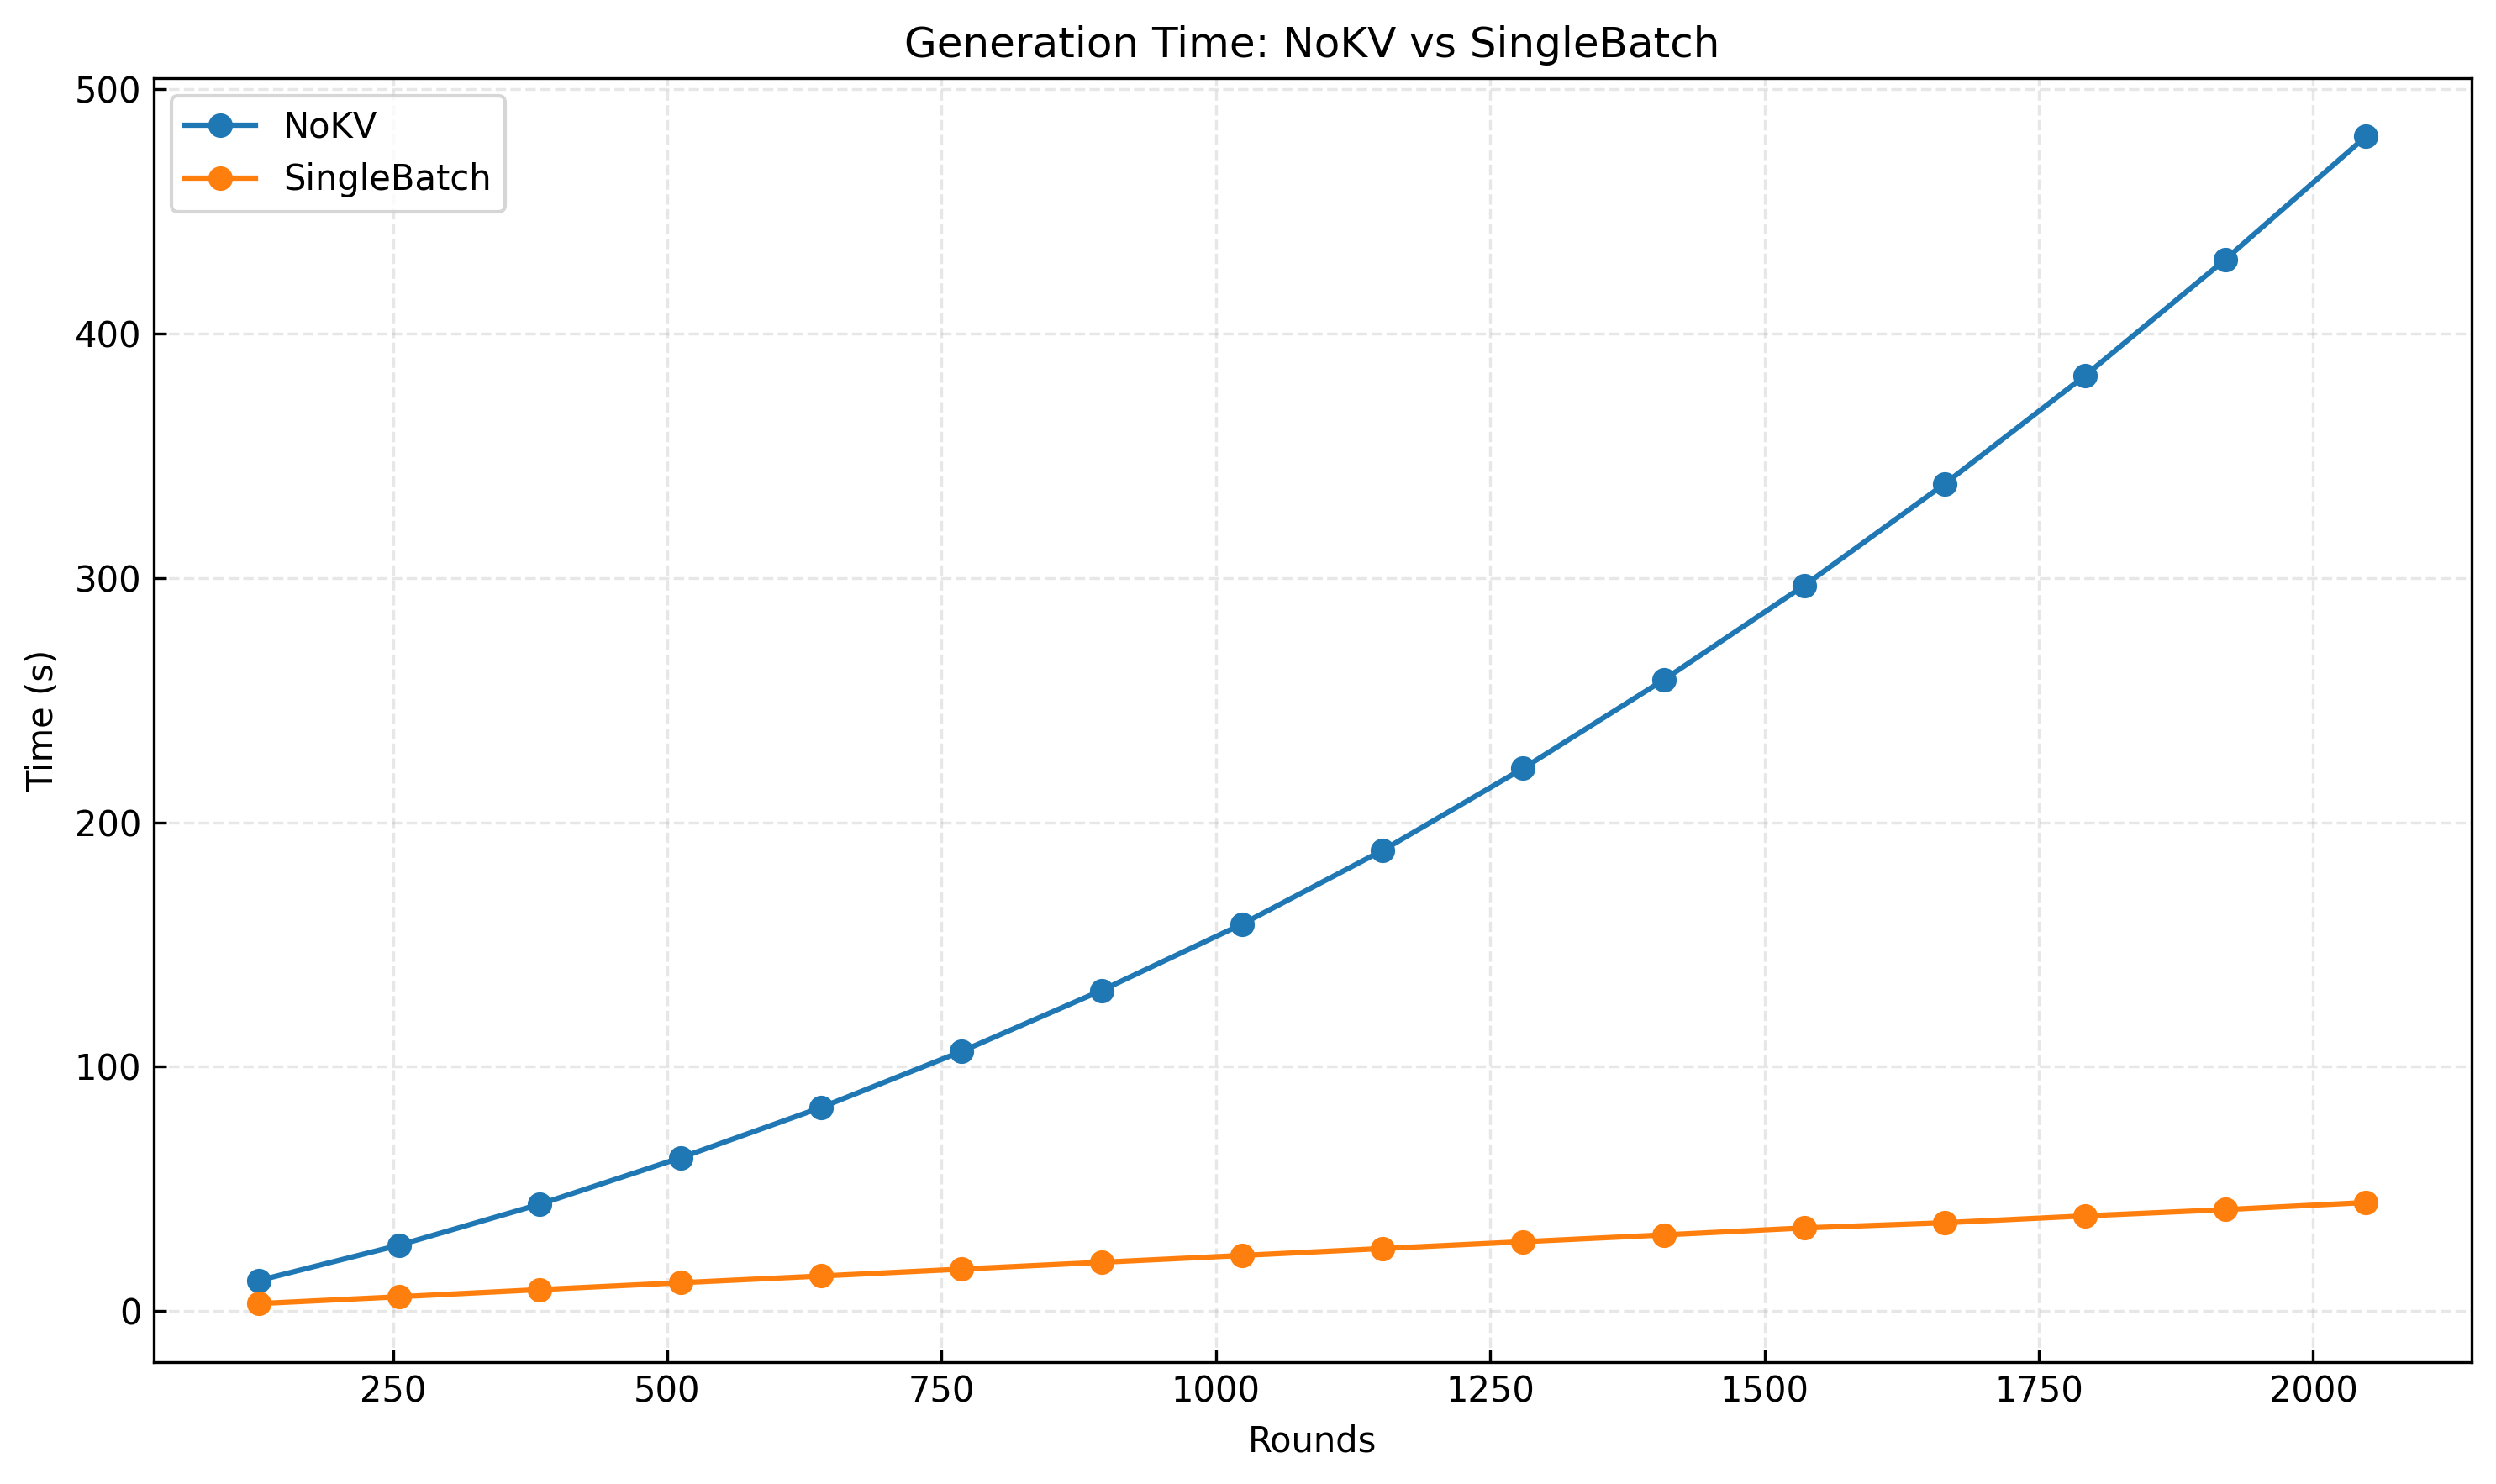
\includegraphics[width=1\linewidth]{fig/hw2-s2-q1.png}
        \caption{Demonstrating the efficiency of deploying KV cache.}
        \label{fig:cache}
        \end{figure}

        \item Compare two implementations: the original implementation without KV cache, and your implementation with KV cache. What trends do you observe in the generation time as the output length increases in both cases? \\

        Without the KV cache implementation, the generation time increases exponentially $\mathcal{O}\left(n^2\right)$ as a function of output length. With the KV cache, the generation time increases linearly $\mathcal{O}\left(n\right)$ as a function of output length. 

    \end{enumerate}

    \item 
    \begin{enumerate}
        \item Extend your KV cache implementation to handle a batch of requests in \texttt{uniform\_prefill.py}, assuming the prompts have the same length. Extend your KV cache implementation to handle a batch of requests in \texttt{different\_prefill.py}, assuming the prompts have different lengths. Profile the end-to-end generation time (only consider the generation, exclude model loading and other overheads) with a batch size of $2^0$ to $2^6$. Each request has an input length of 512 and an output length of 128. Compute the throughput token/s for different batch sizes. Plot the generation time vs batch size and the throughput vs batch size.

        \begin{figure}[H]
        \centering
        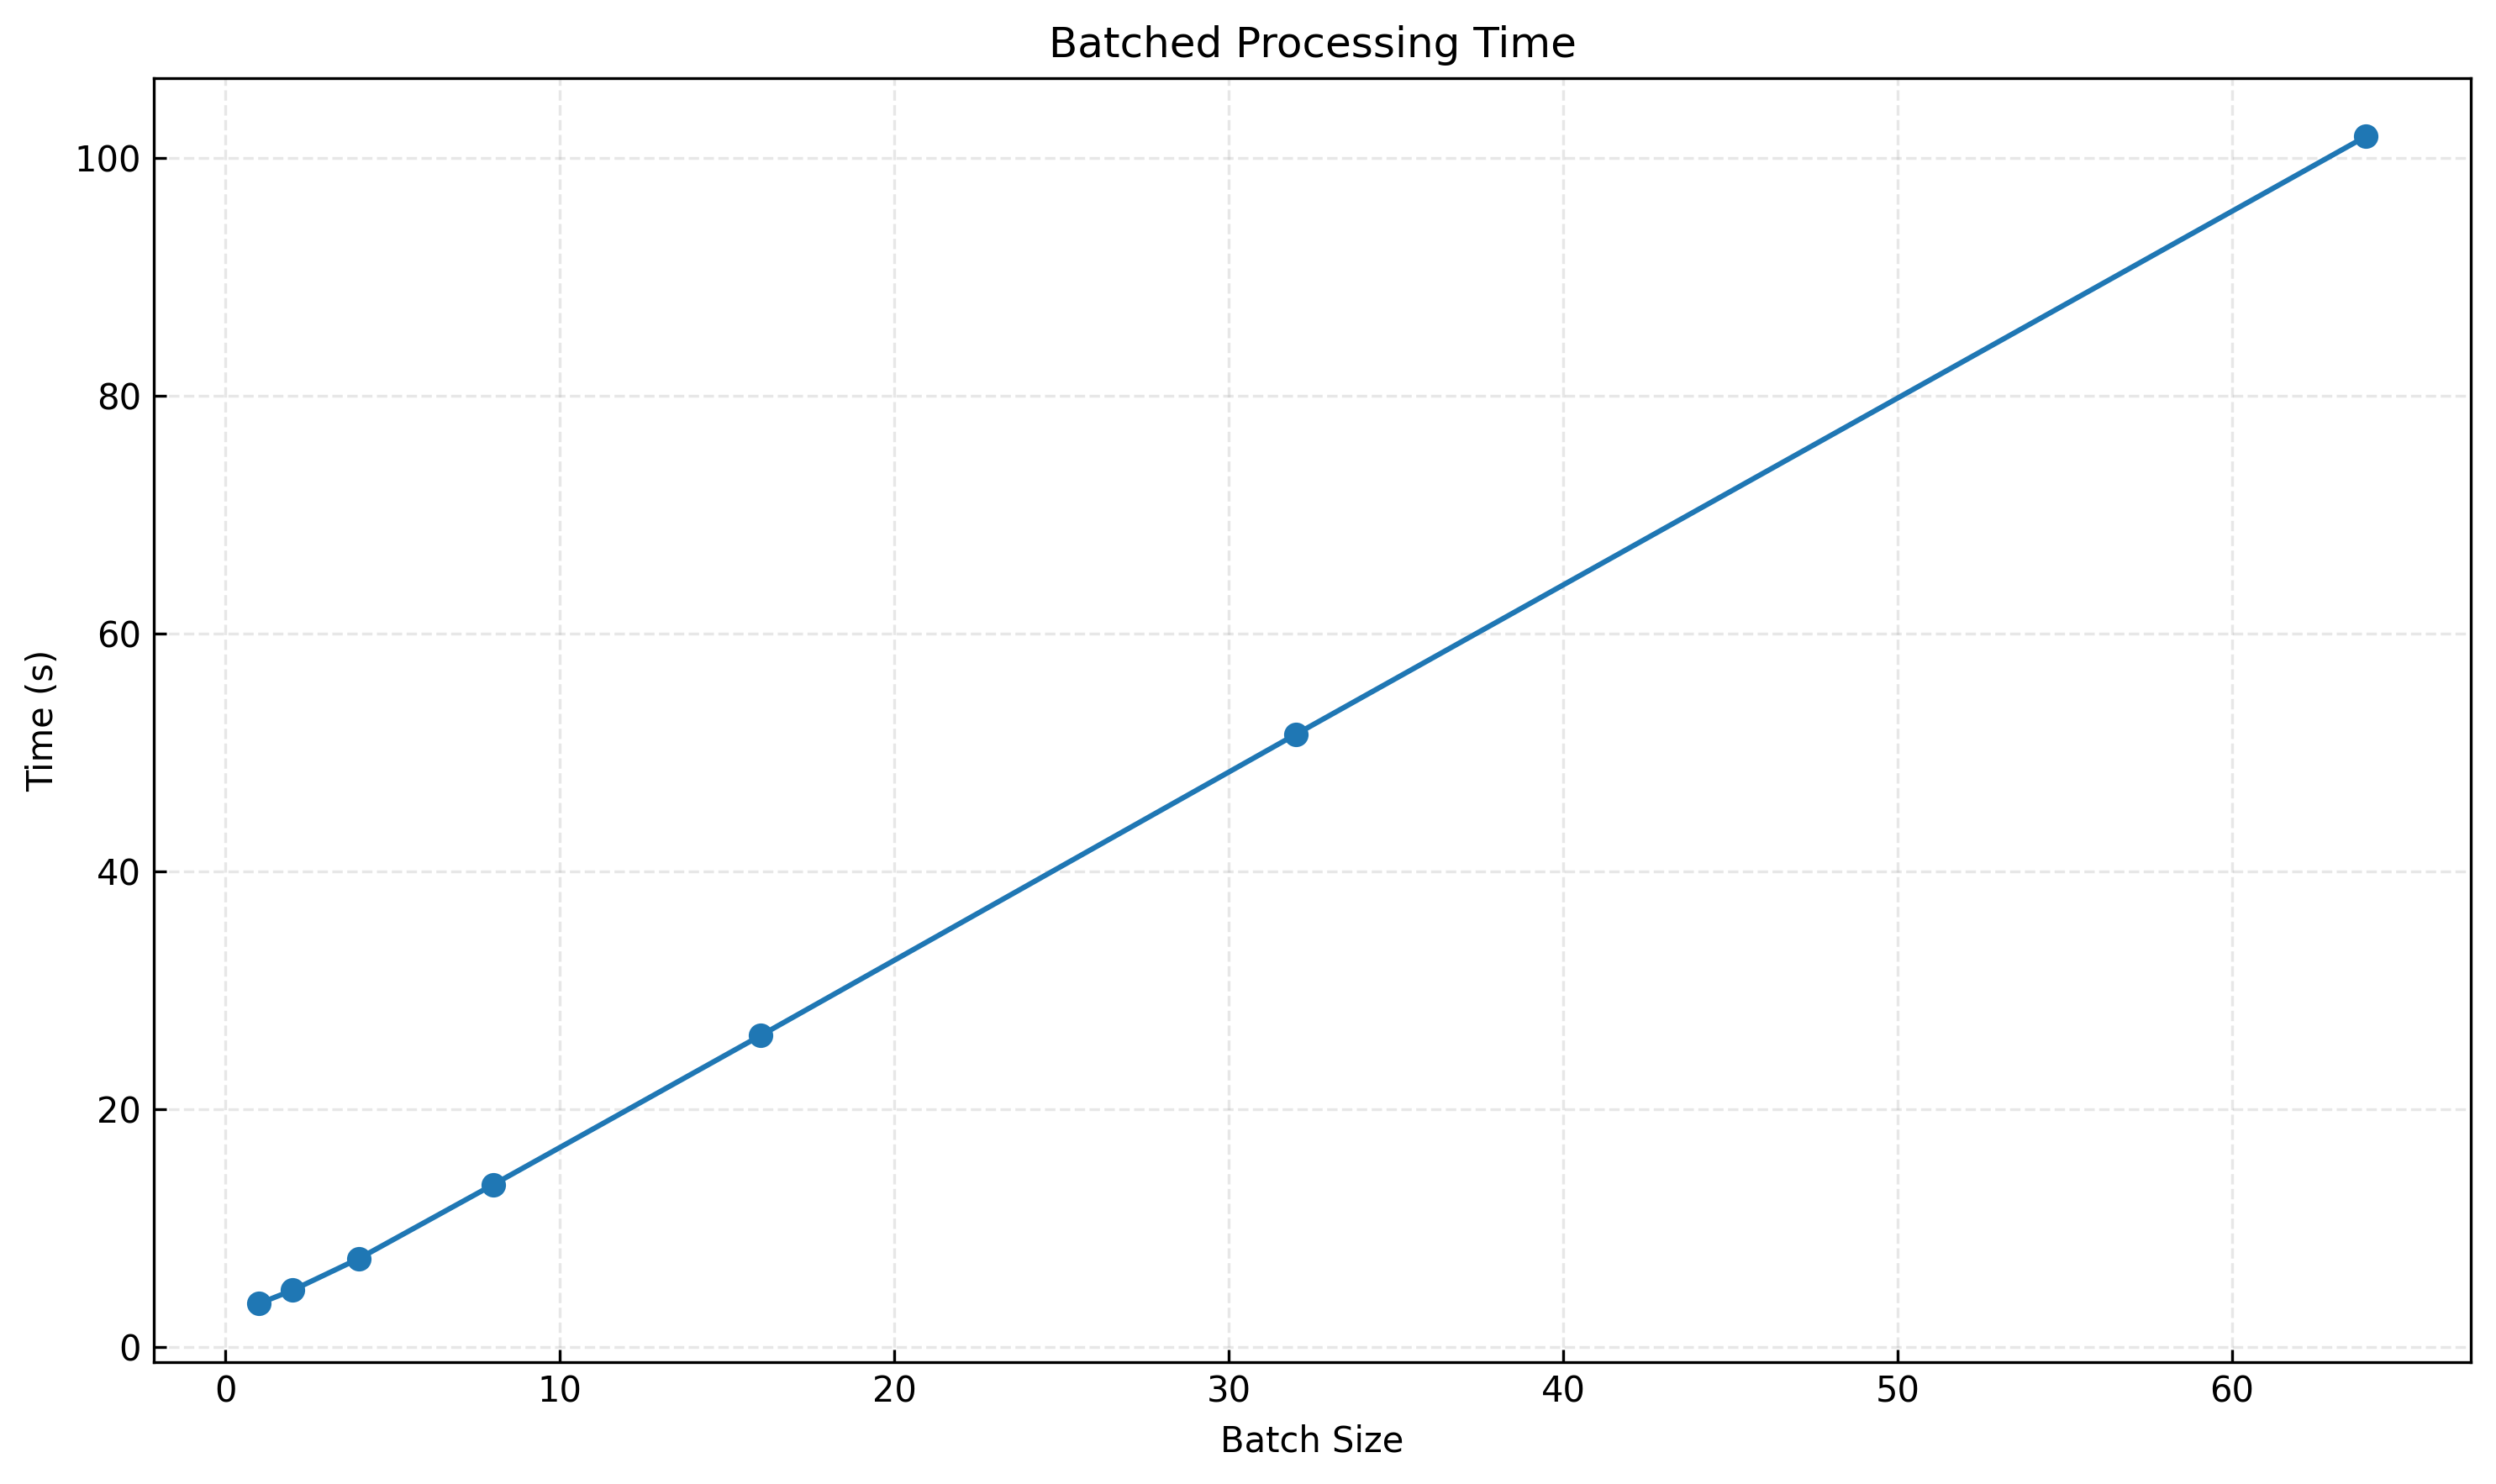
\includegraphics[width=1\linewidth]{fig/hw2-s2-q2-time.png}
        \caption{Demonstrating the efficiency of batched KV cache as measured by generation time.}
        \label{fig:batched-time}
        \end{figure}

        \begin{figure}[H]
        \centering
        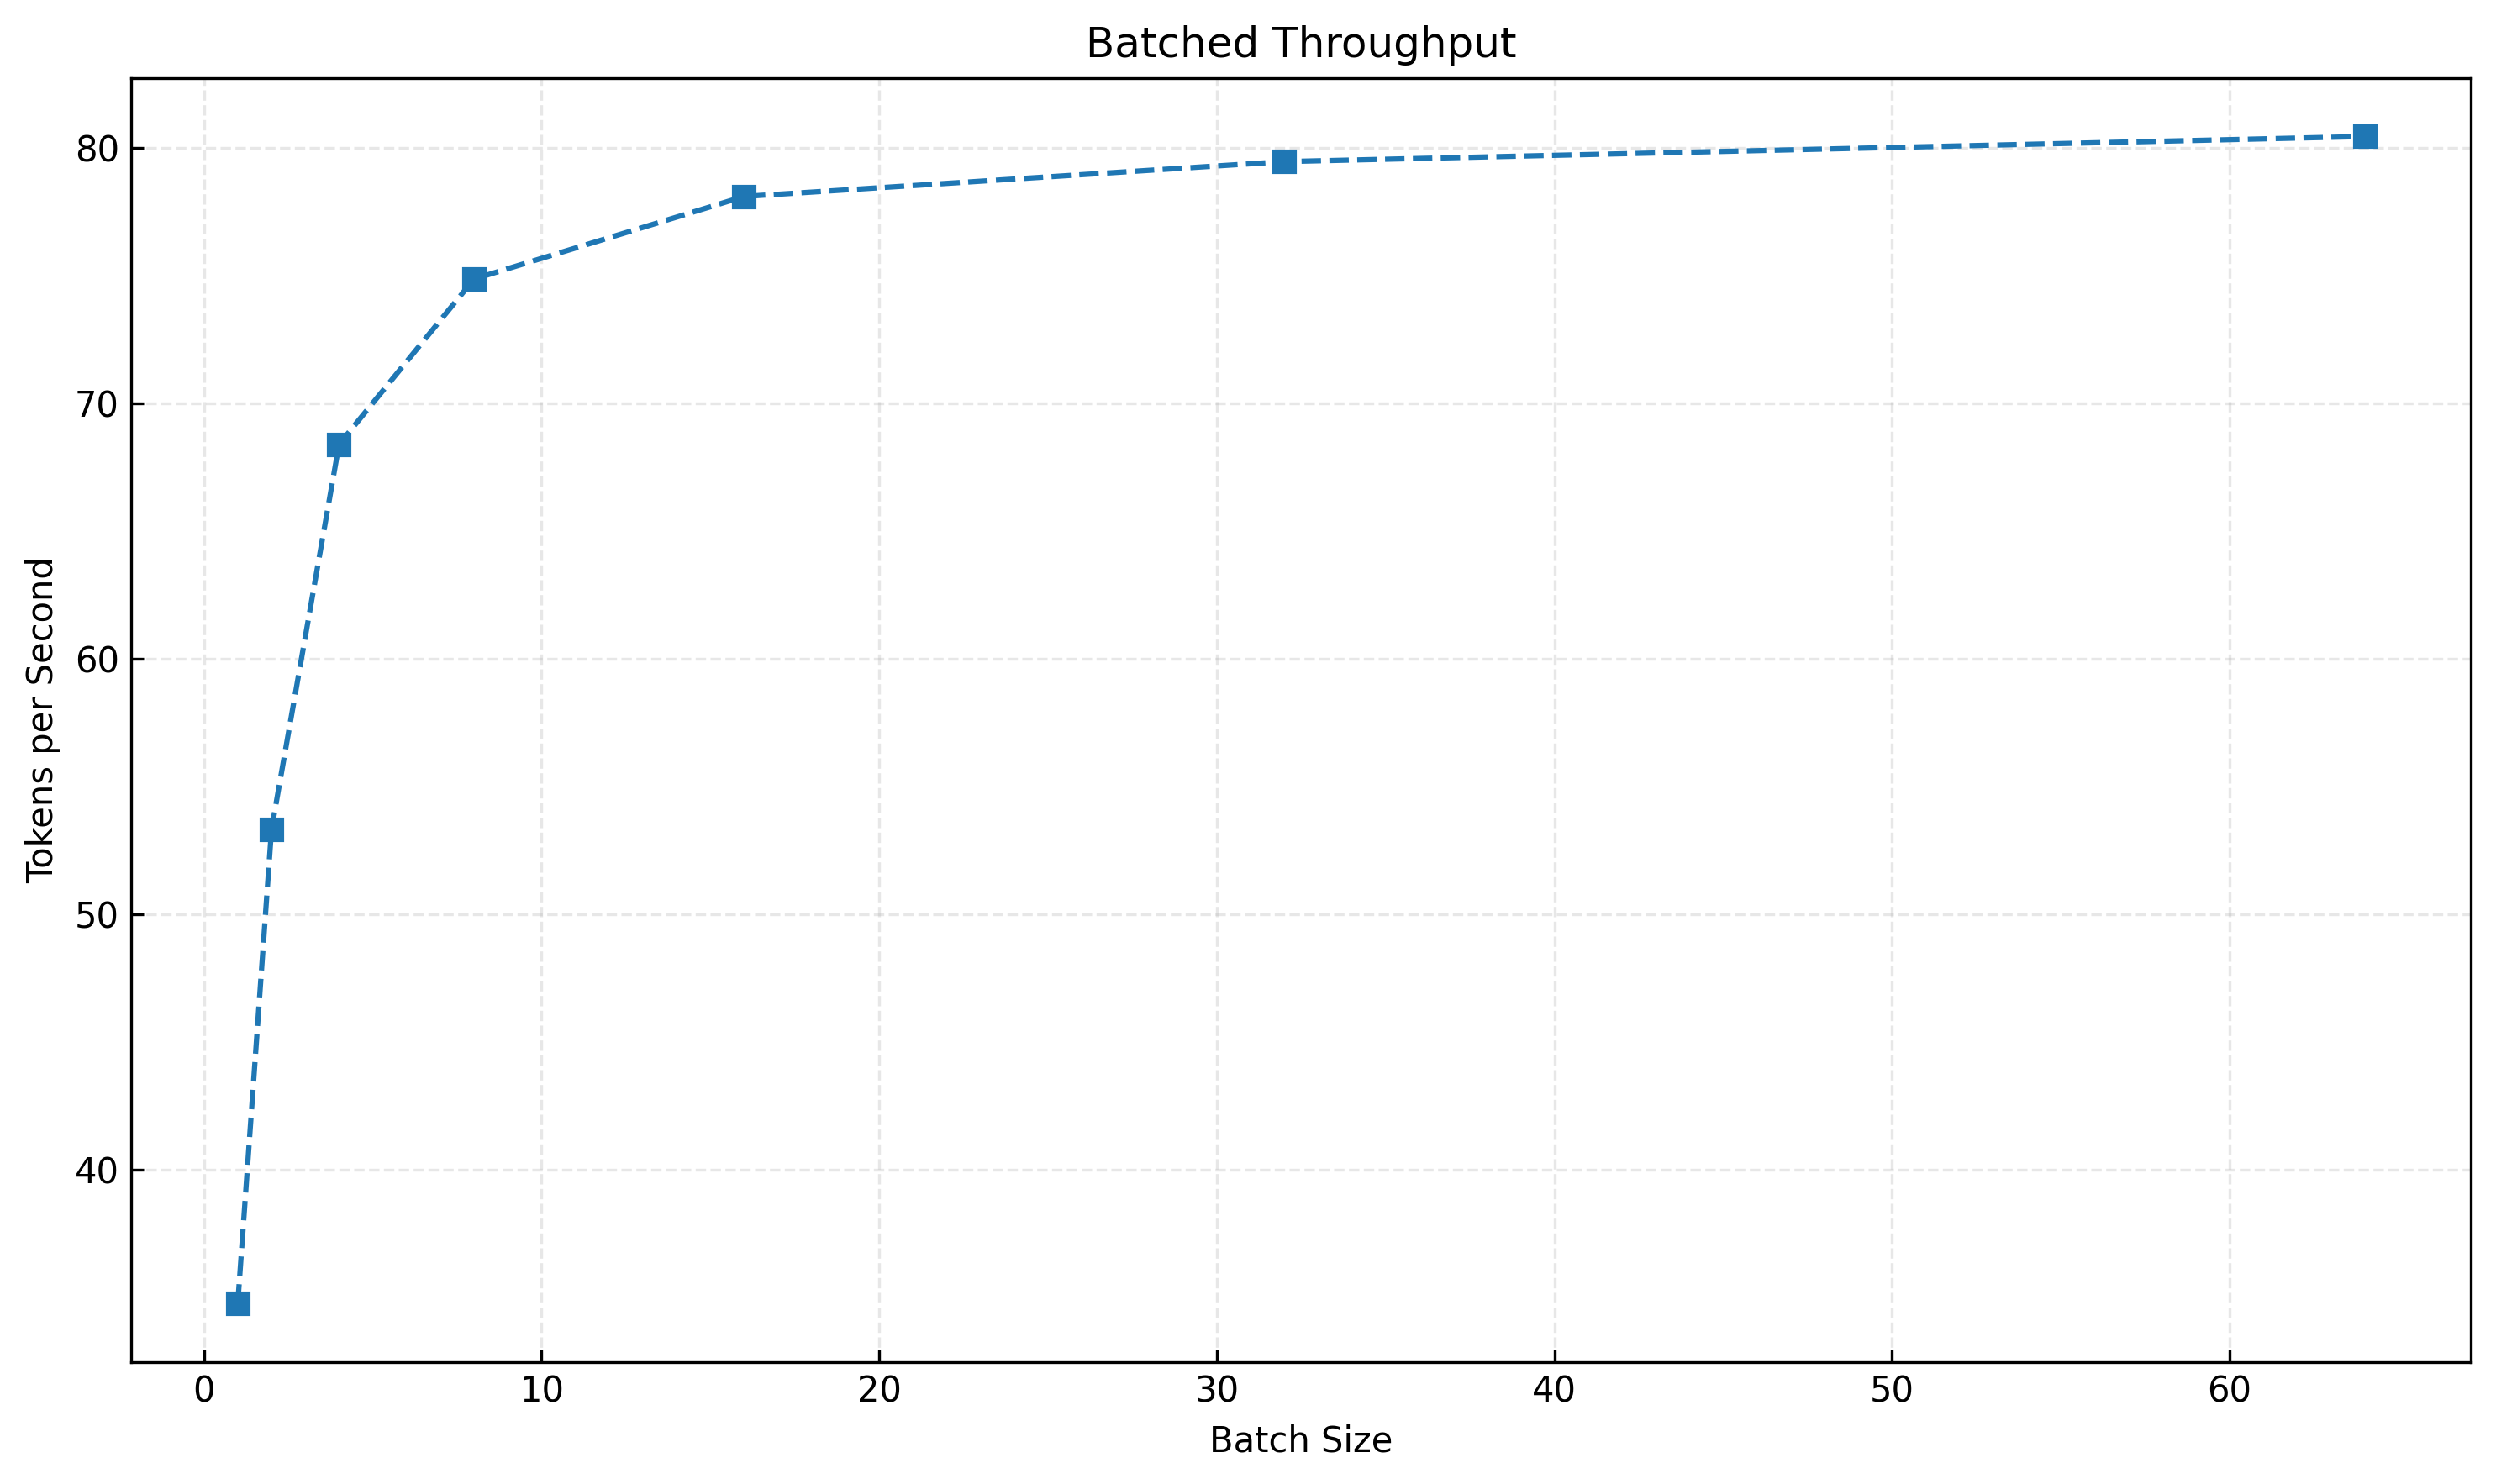
\includegraphics[width=1\linewidth]{fig/hw2-s2-q2-throughput.png}
        \caption{Demonstrating the throughput of the batched KV cache implementation as measured by tokens per second.}
        \label{fig:batched-tps}
        \end{figure}

        \item What trend do you observe? Why is this the case? \\
        
        The processing time continues to increase linearly as a function of batch size (Figure \ref{fig:batched-time}). The other trend observed is that batch processing of sequences with KV cache rapidly increases the throughput, as measured by tokens generated per second (Figure \ref{fig:batched-tps}). However, the rise in throughput quickly plateaus as a result of other bottlenecks being introduced, presumably the ability of compute to process the data stored in GPU memory. Ultimately, an ideal batch size is around $2^4$ to balance throughput and run time before diminishing returns are observed.

    \end{enumerate}
\end{enumerate}

\printbibliography

\end{document}